\section{Kết quả và đánh giá}
\label{sec:evaluation}

\subsection{Hiệu lực phát hiện ngoại tuyến trên DongTing}

\subsubsection{Hiệu năng từng mô hình và tập hợp}
Bảng~\ref{tab:offline} trình bày kết quả trên tập kiểm tra DongTing (lấy trực tiếp
từ \texttt{results.json}). VAE đạt AUC kiểm định cao và ổn định qua ba hạt giống
($0{,}9426$ / $0{,}9438$ / $0{,}9430$; chọn hạt giống~1). Trên tập kiểm tra, tập
hợp đạt AUC $0{,}835$ và Average Precision $0{,}990$.

\begin{table}[htbp]
  \centering
  \caption{Hiệu năng SyscallAD trên tập kiểm tra DongTing (cửa sổ $15/3$, 43 chiều).
           Ngưỡng chọn trên tập kiểm định.}
  \label{tab:offline}
  \begin{tabular}{lccccc}
    \toprule
    \textbf{Mô hình} & \textbf{AUC} & \textbf{AP} & \textbf{F1} & \textbf{Precision} & \textbf{Recall} \\
    \midrule
    iForest          & 0{,}851 & 0{,}991 & 0{,}474 & 0{,}999 & 0{,}311 \\
    VAE              & 0{,}734 & 0{,}985 & 0{,}421 & 0{,}999 & 0{,}267 \\
    \textbf{Tập hợp} & \textbf{0{,}835} & \textbf{0{,}990} & \textbf{0{,}417} & \textbf{0{,}999} & \textbf{0{,}264} \\
    \midrule
    VAE (AUC kiểm định, hạt giống tốt nhất) & 0{,}944 & --- & --- & --- & --- \\
    \bottomrule
  \end{tabular}
\end{table}

\subsubsection{Đối chiếu với công trình tham chiếu}
Bảng~\ref{tab:compare} đối chiếu kết quả của cơ chế đề xuất với mức công bố của
công trình tham chiếu DeSFAM~\cite{desfam_original}. Có \emph{tương đồng} ở hai
điểm: (i) AUC kiểm định của VAE thậm chí cao hơn mức công bố cho thành phần VAE;
(ii) độ chính xác (precision) rất cao ($\approx 0{,}999$), khớp định hướng ``ít báo
động giả''. Tuy nhiên \emph{còn khác biệt} ở F1/Recall so với mức công bố: F1 tập
hợp của chúng tôi
$0{,}417$ so với $0{,}92$ trong công trình tham chiếu, do recall thấp ($0{,}264$) tại ngưỡng bảo
thủ chọn trên tập kiểm định (ngưỡng ưu tiên precision). Nói cách khác, mô hình
\emph{xếp hạng} bất thường tốt (AUC/AP cao) nhưng \emph{điểm chốt nhị phân} tại
một ngưỡng cố định lại bỏ sót nhiều cửa sổ tấn công.

\begin{table}[htbp]
  \centering
  \caption{Cơ chế đề xuất so với số liệu công bố của công trình tham chiếu DeSFAM
           (lõi phát hiện bất thường).}
  \label{tab:compare}
  \begin{tabular}{lcc>{\raggedright\arraybackslash}p{4.2cm}}
    \toprule
    \textbf{Chỉ số} & \textbf{DeSFAM (công bố)} & \textbf{Cơ chế đề xuất} & \textbf{Nhận định} \\
    \midrule
    AUC (tập hợp)        & 0{,}94 & 0{,}835 & Thấp hơn nhưng cùng bậc \\
    AP                   & 0{,}87 & 0{,}990 & Cao hơn (dữ liệu mất cân bằng) \\
    F1 (tấn công)        & 0{,}92 & 0{,}417 & \textbf{Còn khác biệt}---do ngưỡng ưu tiên precision \\
    VAE (AUC kiểm định)  & 0{,}747\,$^{*}$ & 0{,}944 & Cao hơn mức công bố cho VAE \\
    Precision            & cao    & 0{,}999 & Tái lập định hướng ít báo động giả \\
    \bottomrule
    \multicolumn{4}{l}{\footnotesize $^{*}$Giá trị thành phần VAE theo Bảng~1 của công trình tham chiếu; tập hợp công bố $\approx 0{,}94$.}
  \end{tabular}
\end{table}

\subsection{Triển khai trực tiếp trên multi-tenant Kubernetes}
Khi phục vụ trực tiếp, mô hình huấn luyện ngoại tuyến giữ được \emph{khả năng phân
tách} giữa lành tính và tấn công---kết quả quan trọng nhất của chuyên đề:
\begin{itemize}[leftmargin=1.6em]
  \item Khối lượng lành tính (MongoDB) có điểm bất thường $\le 0{,}19$.
  \item Các kịch bản tấn công trong không gian tên \texttt{demo} có điểm
        $0{,}278$--$0{,}930$.
\end{itemize}
Khoảng trống giữa hai phân phối cho phép đặt một \textbf{ngưỡng vận hành
$T_0 = 0{,}25$} (lưu trong \texttt{inference/.env.uat}) tách sạch hai lớp trong
môi trường thử nghiệm (Hình~\ref{fig:separation}). Đây là bằng chứng cho thấy
thiết kế DeSFAM khả thi ngoài mô phỏng: cùng một không gian đặc trưng 43 chiều,
sinh ngoại tuyến từ DongTing và trực tuyến từ Tetragon, tạo ra điểm số tương thích.

\begin{figure}[htbp]
  \centering
  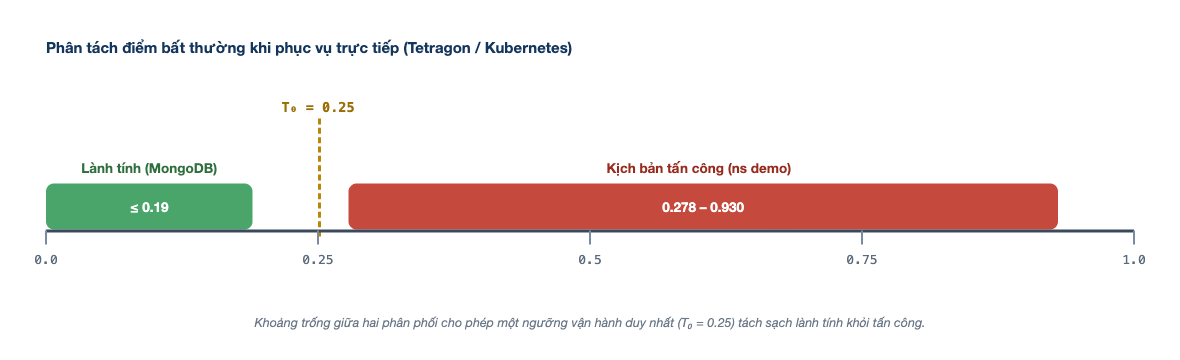
\includegraphics[width=\linewidth]{figures/live-separation}
  \caption{Phân tách điểm bất thường khi phục vụ trực tiếp qua Tetragon trên
           Kubernetes. Khối lượng lành tính (MongoDB) nằm dưới ngưỡng vận hành
           $T_0=0{,}25$, các kịch bản tấn công nằm trên---khoảng trống đủ rộng để
           một ngưỡng duy nhất tách sạch hai lớp.}
  \label{fig:separation}
\end{figure}

\begin{table}[htbp]
  \centering
  \caption{Phân tách điểm bất thường khi phục vụ trực tiếp (Tetragon/K8s).}
  \label{tab:live}
  \begin{tabular}{lcc}
    \toprule
    \textbf{Nguồn} & \textbf{Khoảng điểm} & \textbf{So với $T_0=0{,}25$} \\
    \midrule
    MongoDB (lành tính)        & $\le 0{,}19$        & Dưới ngưỡng (không báo động) \\
    Kịch bản tấn công (\texttt{demo}) & $0{,}278$--$0{,}930$ & Trên ngưỡng (báo động) \\
    \bottomrule
  \end{tabular}
\end{table}

\subsection{Điều kiện thành công của cơ chế}
Yếu tố quyết định là \textbf{căn chỉnh bảng chữ cái cảm biến} giữa huấn luyện và
phục vụ. Khi huấn luyện trên toàn bộ vũ trụ syscall (gồm read/write/close/futex
mật độ cao) trong khi Tetragon chỉ phát 23 syscall an ninh, mọi cửa sổ trực tiếp
trở nên thưa và \emph{suy biến}: điểm lành tính $\approx$ điểm tấn công, không thể
đặt ngưỡng. Sau khi buộc \texttt{train.py} lọc DongTing về đúng 23 syscall trước
khi cắt cửa sổ (\texttt{SENSOR\_ALPHABET=1}), AUC kiểm định của VAE tăng lên
$0{,}944$ (giải quyết sụp đổ hậu nghiệm) và đạt được độ phân tách trực tiếp ở
Bảng~\ref{tab:live}. Bài học: trong các hệ phát hiện bất thường \emph{huấn
luyện-rồi-phục-vụ}, sự đồng nhất không gian đặc trưng quan trọng ngang---thậm chí
hơn---kiến trúc mô hình. Tính đồng nhất này được ràng buộc bằng kiểm thử ngang
hàng \texttt{test\_feature\_parity.py} (đạt) để \texttt{train.py} và bộ trích đặc
trưng khi phục vụ sinh véc-tơ \emph{trùng khít từng bit}.
